% =====================================================================
%  Class Project -- Defense (Blue Team Technical Report)
%  Enterprise Attack-Defense Lab / Group 6
%
%  Compile:  xelatex BLUE_TEAM_REPORT.tex   (run twice for the ToC)
%            or:  tectonic BLUE_TEAM_REPORT.tex
%
%  XeLaTeX is REQUIRED: the author block uses CJK names rendered via
%  xeCJK + Noto Serif CJK.  The body is otherwise English.
% =====================================================================
\documentclass[11pt]{article}

\usepackage{fontspec}
\usepackage{xeCJK}
\setCJKmainfont{Noto Serif CJK TC}
\usepackage[margin=1in]{geometry}
\usepackage{parskip}
\usepackage{booktabs}
\usepackage{tabularx}
\usepackage{array}
\usepackage{enumitem}
\usepackage{xcolor}
\usepackage{listings}
\usepackage{amssymb}
\usepackage{graphicx}
\usepackage{tikz}
\usetikzlibrary{positioning, arrows.meta, fit, backgrounds, calc, shapes.geometric}
\usepackage[hidelinks,colorlinks=true,linkcolor=blue,urlcolor=blue,
            citecolor=blue]{hyperref}

% ---- listings style -------------------------------------------------
\definecolor{codeframe}{gray}{0.55}
\definecolor{codebg}{gray}{0.96}
\lstdefinestyle{blue}{
  basicstyle=\ttfamily\footnotesize,
  breaklines=true,
  breakatwhitespace=false,
  columns=fullflexible,
  keepspaces=true,
  showstringspaces=false,
  frame=single,
  rulecolor=\color{codeframe},
  backgroundcolor=\color{codebg},
  numbers=none,
  xleftmargin=6pt,
  framexleftmargin=6pt,
  framextopmargin=2pt,
  framexbottommargin=2pt,
}
\lstset{style=blue}

% ---- handy inline code macro (escape underscores inside!) -----------
\newcommand{\co}[1]{\texttt{#1}}

\newcolumntype{Y}{>{\raggedright\arraybackslash}X}

% absorb tight lines around long \texttt tokens (avoids overfull boxes)
\emergencystretch=3em

\title{\textbf{Class Project -- Defense}\\[4pt]
       \large Group 6 Hands-on Technical Report (Blue Team)}
\author{%
  M143040024\quad 陳品叡 \\
  M143140012\quad 呂易鴻 \\
  M143140017\quad 王承煜}
\date{2026-06-05}

\begin{document}
\maketitle

\begin{abstract}
\noindent
This report is the defensive companion to our Group~6 attack experiment.
Where the attack report reconstructed an end-to-end Cyber Kill Chain --
reconnaissance, honeypot probing and IP-alias bypass, Flask/Jinja2 SSTI,
fileless ICMP command-and-control, a TCP reverse shell, and DNS/ICMP data
exfiltration -- this document explains \emph{how the Blue Team detects and
responds to each of those behaviors}, what tools implement each control,
and, in detail, \emph{where the defense still fails}.
The defense is organized as two enforcing layers plus a monitoring plane:
(1)~a \textbf{network layer} combining a fake-SSH honeypot with an
\co{iptables} auto-blocker; (2)~a \textbf{kernel layer} built on eBPF that
hooks security-relevant syscalls and can terminate a process in kernel
space \emph{before} the syscall completes; and (3)~a \textbf{SOC dashboard}
that aggregates telemetry from both layers in real time.
We describe the exact detection logic of each eBPF hook (the
fileless-staging detections plus the \co{dup2}/\co{dup3} reverse-shell hook,
all in \co{blue\_ebpf\_mdr\_v2.py}), the cold-start
\co{/proc} scanner, and the kernel-space kill mechanism.
We then give an honest evaluation: behavior-based, source-IP-agnostic
kernel detection is far stronger than IP-based blocking, but it has real
blind spots -- most importantly, covert channels built from
\emph{legitimate} syscalls (DNS/ICMP exfiltration) and persistence
(\co{crontab}) survive the full defense stack. The central lesson is that
defense-in-depth is a continuous process, not a finished product.
\end{abstract}

\tableofcontents

% =====================================================================
\section{Introduction}
% =====================================================================

\subsection{Project context}
The project implements a self-contained red--blue lab (target service,
honeypot, eBPF detection, C2, and exfiltration) that walks the full Cyber
Kill Chain and maps each step to MITRE ATT\&CK. The attack report
(Hands-on~2) documented the offensive path. \textbf{This report takes the
defender's seat}: it describes the controls the Blue Team operates, the
order in which they are brought online, the evidence each one produces, and
the residual risk that remains after every control is running. The red team
is referenced only where it is needed to explain \emph{what} a given control
is defending against.

\subsection{Defensive methodology}
We follow three principles.
\begin{enumerate}[leftmargin=1.4em]
  \item \textbf{Defense in depth.} No single control is treated as a
        complete stop. Each layer is expected to fail against some class of
        attack; the point of layering is that the next layer catches what
        the previous one missed.
  \item \textbf{Behavior over signature.} The kernel layer does not match
        file hashes or IP reputation; it matches \emph{actions}
        (syscalls and their arguments). This is what lets it catch fileless
        malware that never touches disk and survives an attacker changing
        source IP.
  \item \textbf{Evidence-driven, code-accurate.} Every claim about what a
        control does is taken from the tool source, not from the demo
        script. Where the demo narrative and the code disagree, we describe
        the code's actual behavior and flag the difference
        (see \S\ref{sec:connectkill}).
\end{enumerate}

\subsection{Objectives}
\begin{enumerate}[leftmargin=1.4em]
  \item Describe the Blue Team architecture and the role of every defensive
        component.
  \item Document the detection-and-response \emph{workflow}: how telemetry
        flows from sensors to the SOC, and how the operator drives the
        controls round by round.
  \item Give a precise, accurate account of each eBPF hook and the
        kernel-space kill mechanism.
  \item Critically evaluate the limitations -- what gets through, why, and
        what would be required to close each gap.
\end{enumerate}

\subsection{Scope and ethics}
All activity ran in an isolated lab with explicit authorization for
education. The target is purpose-built for the course. The defensive tools
(honeypot, network MDR, eBPF MDR, SOC dashboard) are general-purpose
detection code; nothing here is intended for, or safe to run against,
systems you do not own.

% =====================================================================
\section{Threat Model and Defensive Frame}
% =====================================================================

\subsection{What we are defending against}
From the defender's point of view, the relevant attacker behaviors --
abstracted away from the specific exploit -- are:
\begin{itemize}[leftmargin=1.4em]
  \item \textbf{Probing / target selection} against exposed services.
  \item \textbf{Application-layer code execution} (SSTI) that turns a web
        request into arbitrary Python on the host.
  \item \textbf{Fileless staging}: code is created as an anonymous in-memory
        file descriptor (\co{memfd\_create}) and executed via
        \co{/proc/<pid>/fd/<N>}, leaving no file on disk to scan.
  \item \textbf{Covert command-and-control}: control traffic hidden inside
        ICMP echo payloads (encrypted), or a plain TCP reverse shell.
  \item \textbf{Data exfiltration} over alternative protocols (Base32-over-DNS,
        hex-over-ICMP).
  \item \textbf{Persistence} via \co{crontab} that re-downloads the agent.
\end{itemize}

\subsection{Defense-in-depth model}
The controls form two enforcing layers under one monitoring plane
(Figure~\ref{fig:did}).

\begin{figure}[ht]
\centering
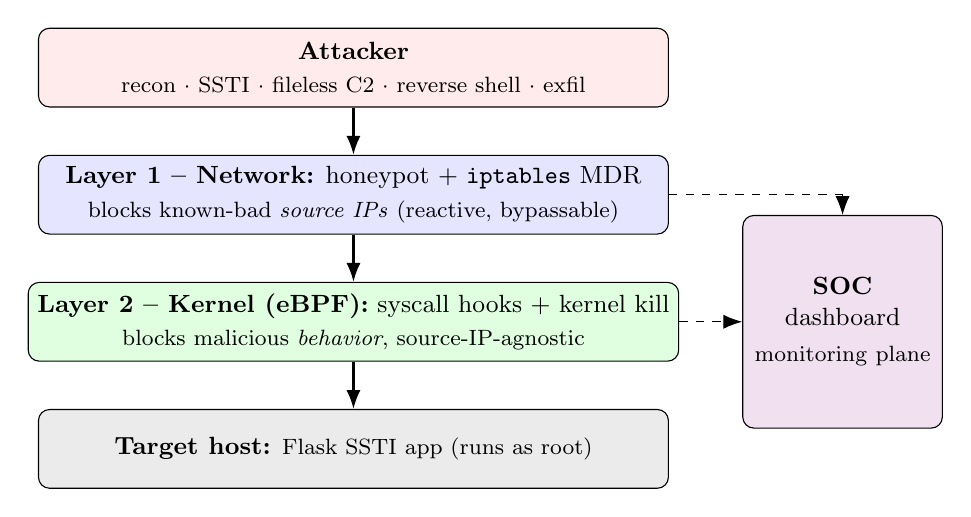
\begin{tikzpicture}[font=\small,
  band/.style={draw, rounded corners, minimum width=8cm, minimum height=1.0cm,
               align=center},
  >={Latex[length=2.4mm]}]
  \node[band, fill=red!8] (atk)
        {\textbf{Attacker}\\[1pt]\footnotesize recon $\cdot$ SSTI $\cdot$
         fileless C2 $\cdot$ reverse shell $\cdot$ exfil};
  \node[band, fill=blue!10, below=6mm of atk] (l1)
        {\textbf{Layer 1 -- Network:} honeypot $+$ \texttt{iptables} MDR\\[1pt]
         \footnotesize blocks known-bad \emph{source IPs} (reactive, bypassable)};
  \node[band, fill=green!12, below=6mm of l1] (l2)
        {\textbf{Layer 2 -- Kernel (eBPF):} syscall hooks $+$ kernel kill\\[1pt]
         \footnotesize blocks malicious \emph{behavior}, source-IP-agnostic};
  \node[band, fill=black!8, below=6mm of l2] (host)
        {\textbf{Target host:} \footnotesize Flask SSTI app (runs as root)};
  \draw[->,thick] (atk) -- (l1);
  \draw[->,thick] (l1)  -- (l2);
  \draw[->,thick] (l2)  -- (host);
  \node[draw, rounded corners, fill=violet!12, align=center, text width=2.3cm,
        minimum height=2.7cm, right=8mm of l2] (soc)
        {\textbf{SOC}\\ dashboard\\[2pt]\footnotesize monitoring plane};
  \draw[->,dashed] (l1.east) -| (soc.north);
  \draw[->,dashed] (l2.east) -- (soc.west);
\end{tikzpicture}
\caption{Defense-in-depth. Each layer is expected to fail against some class
of attack; the next layer---and the SOC monitoring plane---watches the gap.
Solid arrows = attack progression; dashed = telemetry to the SOC.}
\label{fig:did}
\end{figure}

The ordering matters: Layer~1 is cheap, generates early signal, and buys
time, but is trivially bypassed (\S\ref{sec:net-limits}); Layer~2 is the
real enforcement point because it acts on behavior the attacker cannot avoid
if they want code execution and a control channel.

\subsection{Detection coverage (MITRE ATT\&CK)}
\label{sec:coverage}
Table~\ref{tab:coverage} maps each attacker technique to the control that
detects it, the layer, and whether that control \emph{enforces}
(kills/blocks) or only \emph{alerts}. The enforce-vs-alert column is
important and is justified per-hook in \S\ref{sec:kernel}.

\begin{table}[h]
\centering
\caption{Detection-and-response coverage. ``Enforce'' = the control can stop
the action; ``Alert'' = the control records it but does not stop it.}
\label{tab:coverage}
\small
\begin{tabularx}{\linewidth}{@{}l Y l l l@{}}
\toprule
\textbf{ATT\&CK} & \textbf{Technique} & \textbf{Control / hook} & \textbf{Layer} & \textbf{Action}\\
\midrule
T1595 & Active Scanning & Honeypot (\co{honeypot.py}) & Network & Alert\\
--    & (response)      & \co{iptables} MDR & Network & Enforce (block IP)\\
T1190 & Exploit Public-Facing App & (not directly detected) & -- & Gap\\
T1620 & Reflective Code Loading & \co{sys\_enter\_memfd\_create} & Kernel & Alert + taint\\
T1059 & Exec from \co{/proc/fd} & \co{sys\_enter\_execve} (argv) & Kernel & Enforce (kill)\\
T1095 & Non-App-Layer (ICMP) & \co{sys\_enter\_socket} (raw ICMP) & Kernel & Enforce if correlated\\
T1571 & Non-Standard Port & \co{sys\_enter\_connect} & Kernel & Alert\\
T1059.006 & Reverse-shell fd hijack & \co{sys\_enter\_dup2/dup3} & Kernel & Enforce (kill)\\
T1048.003 & Exfil over DNS/ICMP & (not detected) & -- & Gap\\
T1053.003 & Persistence: Cron & (not detected) & -- & Gap\\
\bottomrule
\end{tabularx}
\end{table}

The three ``Gap'' rows are not oversights; they are the honest boundary of
this defense and are analyzed in \S\ref{sec:limits}.

% =====================================================================
\section{Defensive Architecture and Environment}
% =====================================================================

\subsection{Machines and roles}
Two native Ubuntu~24.04 machines are used. The \textbf{lab machine} hosts the
target service \emph{and} the entire Blue Team stack; the \textbf{attacker
machine} runs the red-team tooling. Only the lab machine needs eBPF and root.

\begin{center}
\begin{tabularx}{\linewidth}{@{}l l Y@{}}
\toprule
\textbf{Machine} & \textbf{Role} & \textbf{Runs}\\
\midrule
Lab & Target + Blue Team & target app, honeypot, eBPF MDR, network MDR, SOC dashboard\\
Attacker & Red Team & recon, C2, reverse shell, exfil (out of scope here)\\
\bottomrule
\end{tabularx}
\end{center}

\subsection{Defensive components}
\begin{table}[h]
\centering
\caption{Blue Team components and their function.}
\label{tab:components}
\small
\begin{tabularx}{\linewidth}{@{}l l Y@{}}
\toprule
\textbf{File} & \textbf{Layer} & \textbf{Function}\\
\midrule
\co{target/honeypot.py} & Network & Fake SSH on :2222; logs every connector IP to \co{trap.log}\\
\co{blue\_team/blue\_mdr\_network.py} & Network & Watches \co{trap.log}; \co{iptables -j DROP} on new IPs\\
\co{blue\_team/blue\_ebpf\_mdr\_v2.py} & Kernel & eBPF MDR: memfd/execve/raw-ICMP staging detection $+$ correlation, connect (suspect ports), dup2/dup3 reverse-shell\\
\co{blue\_team/soc\_dashboard.py} & Monitoring & Flask + SSE timeline over \co{trap.log} and \co{soc\_events.jsonl}\\
\co{cleanup.sh} & Ops & Resets processes, \co{iptables}, IP aliases, logs, crontab\\
\bottomrule
\end{tabularx}
\end{table}

\subsection{Telemetry and data flow}
\label{sec:telemetry}
There are two log sinks, both at the project root, and one in-kernel buffer:

\begin{itemize}[leftmargin=1.4em]
  \item \co{trap.log} -- written by the honeypot, one line per connection,
        in the form \co{[ts] Attacker IP: <ip> Port: <p> Data: <...>}. It is
        the contract between the honeypot and the network MDR.
  \item \co{soc\_events.jsonl} -- one JSON object per line, written by the
        eBPF MDR (kill/alert events) and by the network MDR (IP blocks).
  \item \textbf{perf ring buffer} -- a lock-free, \co{mmap}-shared buffer the
        eBPF program writes and the Python userspace reads (\co{page\_cnt=64},
        i.e.\ 256\,KB).
\end{itemize}

\noindent
Figure~\ref{fig:flow} shows how the sinks are fed and consumed: three
producers write two files, and the SOC dashboard tails both.

\begin{figure}[ht]
\centering
\resizebox{\linewidth}{!}{%
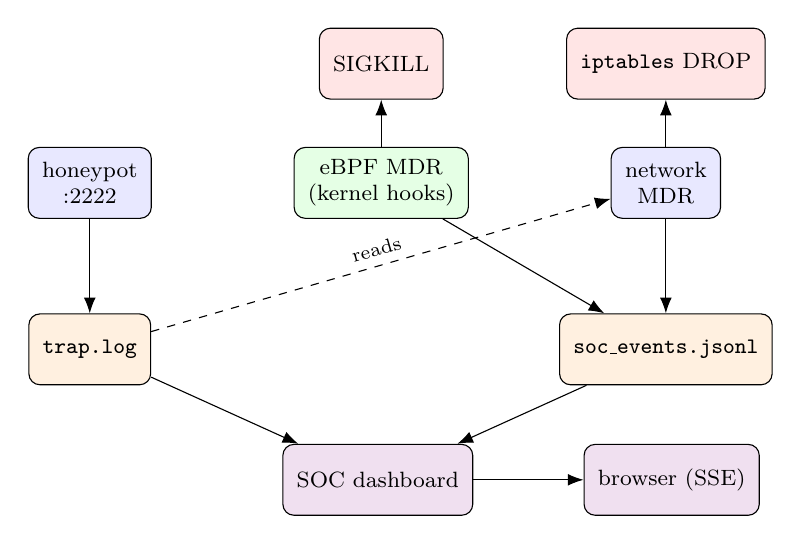
\begin{tikzpicture}[font=\footnotesize, >={Latex[length=2mm]},
  base/.style={draw, rounded corners, align=center, minimum height=0.9cm,
               inner xsep=5pt},
  file/.style={base, fill=orange!12}, act/.style={base, fill=red!10},
  soc/.style={base, fill=violet!12}]
  % producers (top row)
  \node[base, fill=blue!9] (hp) {honeypot\\ :2222};
  \node[base, fill=green!10, right=18mm of hp] (kmdr) {eBPF MDR\\ (kernel hooks)};
  \node[base, fill=blue!9, right=18mm of kmdr] (nmdr) {network\\ MDR};
  % enforcement actions (side effects)
  \node[act, above=6mm of kmdr] (sig) {SIGKILL};
  \node[act, above=6mm of nmdr] (ipt) {\texttt{iptables} DROP};
  % files (middle row)
  \node[file, below=12mm of hp]   (trap)  {\texttt{trap.log}};
  \node[file, below=12mm of nmdr] (jsonl) {\texttt{soc\_events.jsonl}};
  % soc (bottom)
  \coordinate (mid) at ($(trap)!0.5!(jsonl)$);
  \node[soc, below=12mm of mid] (soc) {SOC dashboard};
  \node[soc, right=14mm of soc] (br) {browser (SSE)};
  % edges
  \draw[->] (hp) -- (trap);
  \draw[->,dashed] (trap) -- node[above,sloped,font=\scriptsize]{reads} (nmdr);
  \draw[->] (kmdr) -- (jsonl);
  \draw[->] (nmdr) -- (jsonl);
  \draw[->] (kmdr) -- (sig);
  \draw[->] (nmdr) -- (ipt);
  \draw[->] (trap)  -- (soc);
  \draw[->] (jsonl) -- (soc);
  \draw[->] (soc)   -- (br);
\end{tikzpicture}}
\caption{Telemetry flow. Producers (honeypot, kernel eBPF MDR, network MDR)
write two sinks (\texttt{trap.log}, \texttt{soc\_events.jsonl}); the SOC
dashboard tails both and streams them to the browser over SSE. Enforcement
(SIGKILL, \texttt{iptables} DROP) is a side effect, not telemetry.}
\label{fig:flow}
\end{figure}

% =====================================================================
\section{Layer 1 -- Network-Layer Defense}
% =====================================================================

\subsection{Deception: the fake-SSH honeypot}
The honeypot listens on TCP~2222 and, on every connection, sends a banner
that is byte-for-byte a real OpenSSH version string:
\begin{lstlisting}
SSH-2.0-OpenSSH_8.9p1 Ubuntu-3ubuntu0.4
\end{lstlisting}
To \co{nmap -sV} this is indistinguishable from a genuine SSH service, so a
scanner is drawn to it. The server then reads whatever the client sends
(its SSH client hello), returns a fake ``Permission denied'' rejection, and
records the connection.

The defensive value is \textbf{a near-zero false-positive signal}: nothing
legitimate has any reason to connect to this port. Any hit is, by
construction, suspicious. Each hit is appended to \co{trap.log} with the
source IP, port, and the first 100 bytes the client sent (useful for later
triage). This maps to detecting reconnaissance (T1595) by \emph{inviting}
it into a monitored trap.

\subsection{Automated response: the network MDR}
\co{blue\_mdr\_network.py} is a small daemon that tails \co{trap.log}.
On startup it seeks to the current end of the file (so stale entries from a
previous run are ignored), then polls (default 1\,s) for new lines. For each
new, valid, not-already-blocked IPv4 address it runs:
\begin{lstlisting}
iptables -I INPUT 1 -s <attacker_ip> -j DROP
\end{lstlisting}
Inserting at position~1 makes the DROP the highest-priority INPUT rule, so
the attacker is cut off from \emph{all} ports on the host -- not just 2222 --
in under a second. The block, the IP, and the action are also written to
\co{soc\_events.jsonl} (\co{source: NETWORK\_MDR, event: IP\_BLOCKED}). With
\co{--cleanup}, every rule the daemon added is removed on exit, so the lab
returns to a clean state.

\subsection{Layer-1 defensive process}
\begin{enumerate}[leftmargin=1.4em]
  \item Operator starts the honeypot and the network MDR (with
        \co{--cleanup}) from the same repo directory, so both resolve the
        \emph{same} \co{trap.log} path.
  \item Attacker probes :2222 (deliberately or via a scan).
  \item Honeypot replies with a real-looking banner and logs the IP.
  \item MDR sees the new line within one poll interval and inserts a DROP.
  \item Attacker's original IP can no longer reach the host on any port.
\end{enumerate}

\subsection{Strengths and limitations of Layer~1}
\label{sec:net-limits}
The honeypot is excellent \emph{signal} (high confidence, low noise) and the
auto-block is fast, but the control is fundamentally \textbf{reactive and
IP-scoped}, which is its undoing:
\begin{itemize}[leftmargin=1.4em]
  \item It only blocks IPs that have \emph{already} touched the trap. An
        attacker who never connects to :2222 is never blocked by this layer.
  \item Blocking is by source IP, and \textbf{source IP is attacker-controlled}.
        In the exercise, the red team simply adds an alias IP
        (\co{ip\_switch.sh}) and continues from a fresh identity --
        the real target on :9999 is reachable again immediately. NAT,
        proxies, and IP rotation generalize this bypass.
\end{itemize}
The conclusion the lab draws is the right one: IP-based blocking is a useful
\emph{first} layer that buys time and produces telemetry, not a standalone
preventive control. That is precisely why a second, behavior-based layer is
required.

% =====================================================================
\section{Layer 2 -- Kernel-Layer Defense (eBPF MDR)}
\label{sec:kernel}
% =====================================================================

\subsection{Why eBPF}
eBPF lets us run a small, verified program inside the kernel, attached to
syscall \emph{tracepoints}. This gives the defender four properties that
userspace agents cannot match:
\begin{itemize}[leftmargin=1.4em]
  \item \textbf{Source-IP-agnostic.} It acts on what a process \emph{does},
        so the Layer-1 IP-alias bypass is irrelevant here.
  \item \textbf{Fileless-visible.} It sees \co{memfd\_create} and
        \co{execve} arguments directly, so in-memory malware that never
        writes a file is still observable.
  \item \textbf{Pre-syscall enforcement.} Hooks fire at \emph{syscall entry}
        (\co{sys\_enter\_*}), before the kernel performs the action. A kill
        here breaks the chain before the dangerous operation completes.
  \item \textbf{Low overhead.} Hash-map lookups are $O(1)$ and the program
        is JIT-compiled to native code by the kernel.
\end{itemize}

\subsection{The eBPF pipeline}
BCC compiles the embedded C to eBPF bytecode with Clang/LLVM at runtime; the
kernel \emph{verifier} proves it is safe (bounded loops, no wild pointers);
the JIT converts it to native x86-64; it is attached to tracepoints; and it
communicates with userspace through the perf ring buffer and shared hash
maps. Two design details follow directly from the verifier: every string
scan is a \emph{bounded} loop (\co{for (i=6; i<20; i++)}), and all userspace
reads go through \co{bpf\_probe\_read\_user[\_str]} with explicit sizes
(Figure~\ref{fig:pipeline}).

\begin{figure}[ht]
\centering
\resizebox{\linewidth}{!}{%
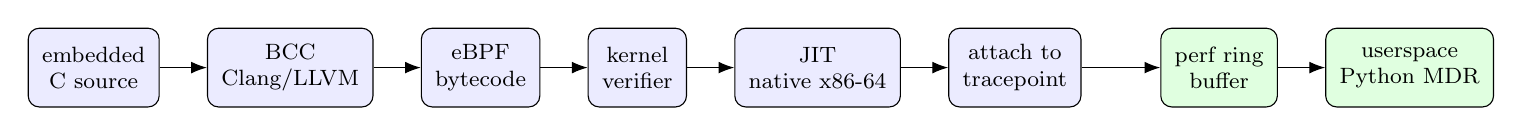
\begin{tikzpicture}[font=\footnotesize, >={Latex[length=2mm]},
  pstep/.style={draw, rounded corners, align=center, minimum height=1cm,
               inner xsep=5pt}]
  \node[pstep, fill=blue!8] (c) {embedded\\ C source};
  \node[pstep, fill=blue!8, right=6mm of c]   (bcc) {BCC\\ Clang/LLVM};
  \node[pstep, fill=blue!8, right=6mm of bcc] (bc)  {eBPF\\ bytecode};
  \node[pstep, fill=blue!8, right=6mm of bc]  (ver) {kernel\\ verifier};
  \node[pstep, fill=blue!8, right=6mm of ver] (jit) {JIT\\ native x86-64};
  \node[pstep, fill=blue!8, right=6mm of jit] (att) {attach to\\ tracepoint};
  \node[pstep, fill=green!12, right=10mm of att] (perf) {perf ring\\ buffer};
  \node[pstep, fill=green!12, right=6mm of perf] (us) {userspace\\ Python MDR};
  \foreach \a/\b in {c/bcc,bcc/bc,bc/ver,ver/jit,jit/att,att/perf,perf/us}
     \draw[->] (\a) -- (\b);
\end{tikzpicture}}
\caption{The eBPF pipeline. Blue = load time (compile, verify, JIT, attach);
green = run time (events surface to userspace through the perf ring buffer).
The verifier is the reason every string scan is a bounded loop.}
\label{fig:pipeline}
\end{figure}

\subsection{Fileless-staging detections}
The eBPF MDR (\co{blue\_ebpf\_mdr\_v2.py}) installs seven probes in total;
the first four target the fileless-staging chain.

\paragraph{Hook 0 -- fork tracking (\co{sched\_process\_fork}).}
When a process that previously called \co{memfd\_create} forks, the child
gets a new PID that the correlation logic would otherwise miss. This hook
copies the parent's entry in the \co{memfd\_pids} map to the child, so the
``memfd taint'' propagates across \co{fork+execve}. Without it, the
correlation in Hook~3 would be defeated by a single fork.

\paragraph{Hook 1 -- \co{memfd\_create} (fileless staging).}
On entry, the hook records \co{(pid, timestamp)} in \co{memfd\_pids} and
captures the anonymous file name. \textbf{It is alert-only}: it never kills
(the kill placeholder is empty in both modes). Its job is to \emph{taint}
the process for later correlation, not to enforce -- \co{memfd\_create} has a
few legitimate users and killing on it alone would be too aggressive.

\paragraph{Hook 2 -- \co{execve} from \co{/proc/<pid>/fd/<N>}.}
This is the actual enforcement point of the fileless chain. The hook
inspects two things:
\begin{itemize}[leftmargin=1.4em]
  \item the \co{execve} \emph{filename}; if it is itself \co{/proc/.../fd/...}
        (used legitimately by systemd's \co{sd-executor}) it is
        \textbf{alert-only};
  \item \co{argv[1]}; if \emph{that} points at \co{/proc/.../fd/...}
        (the pattern \co{python3 /proc/<pid>/fd/<N>} used by the fileless
        loader) it is \textbf{killed}.
\end{itemize}
This filename-vs-argv distinction is a deliberate false-positive control: it
separates a legitimate systemd pattern from the red-team pattern and only
enforces on the latter.

\paragraph{Hook 3 -- raw ICMP socket + correlation.}
The socket hook filters precisely for
\co{socket(AF\_INET, SOCK\_RAW, IPPROTO\_ICMP)}. A standalone raw ICMP
socket (e.g.\ \co{ping}) is \textbf{alert-only}. But if the calling PID
\emph{or its parent} is in \co{memfd\_pids}, we have a high-confidence
correlation -- \emph{fileless staging plus a covert ICMP channel} -- which is
extremely unlikely to be benign, and it is \textbf{killed}. This
multi-indicator correlation is the staging detector's strongest idea: it raises
confidence enough to justify an automated kill.

\subsection{Cold-start \co{/proc} scanner}
\label{sec:coldstart}
eBPF tracepoints only fire on \emph{new} syscalls. If the agent was deployed
\emph{before} the Blue Team started monitoring, the hooks never see it. The
tool compensates with a one-shot \co{/proc} walk at startup that finds
already-running fileless processes two ways:
\begin{enumerate}[leftmargin=1.4em]
  \item \co{/proc/<pid>/exe} resolving to \co{memfd:*} (direct memfd exec);
  \item a \co{python*} process whose \co{argv} references a live
        \co{/proc/<pid>/fd/<N>} that in turn points at a \co{memfd:} target
        (the Python fileless-loader pattern).
\end{enumerate}
With \co{--kill}, matches are terminated with a userspace \co{SIGKILL}. This
is a \emph{compensating} control: it narrows, but does not eliminate, the
temporal gap (\S\ref{sec:gap-limits}).

\subsection{Reverse-shell detection}
A TCP reverse shell uses only ordinary syscalls
(\co{socket(SOCK\_STREAM)} $\to$ \co{connect} $\to$ \co{dup2} $\to$
\co{pty.spawn}), so none of the four staging hooks above fire on it. The
remaining three hooks exist to close that gap.

\paragraph{Hook 4 -- \co{connect} to a suspect port.}
The hook reads the first 8 bytes of the \co{sockaddr} the program passed to
\co{connect}, checks the family is \co{AF\_INET}, byte-swaps the port to host
order, and looks it up in a \co{suspect\_ports} hash map populated from
Python at startup (default \{4444, 4445, 5555, 1234, 1337\}). On a hit it
records the destination IP and port. \textbf{It is alert-only}
(\S\ref{sec:connectkill}).

\paragraph{Hook 5/6 -- \co{dup2} / \co{dup3} fd-hijack.}
A reverse shell redirects all three standard descriptors to the socket:
\co{dup2(s,0)}, \co{dup2(s,1)}, \co{dup2(s,2)}. The hook keeps a per-PID
bitmask; each redirect of fd~0/1/2 sets a bit. When the mask reaches
\co{0x07} (all three), a reverse shell is confirmed and the process is
\textbf{killed}. \co{dup3} is hooked as well because Python's
\co{os.dup2(..., inheritable=False)} actually calls \co{dup3}; without it an
attacker bypasses Hook~5 with one keyword argument. Crucially, this signal
fires \emph{regardless of port}: even a reverse shell on 80/443 (to blend
in) is caught the moment it hijacks the three fds.
Figure~\ref{fig:dup2} shows this as a per-PID bitmask state machine.

\begin{figure}[ht]
\centering
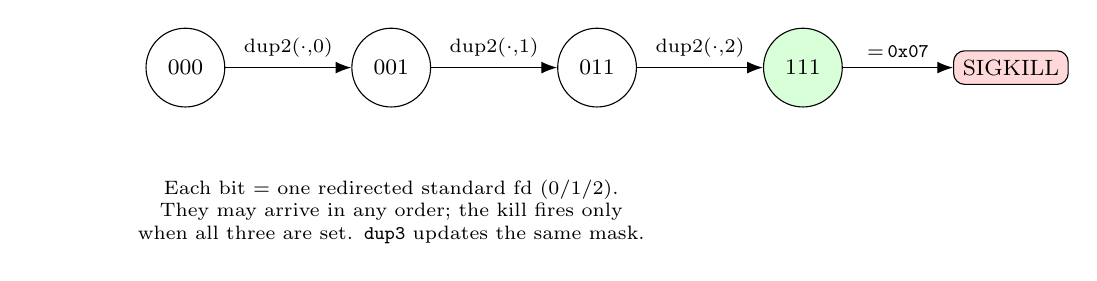
\begin{tikzpicture}[font=\footnotesize, >={Latex[length=2mm]},
  st/.style={draw, circle, minimum size=10mm, inner sep=1pt}]
  \node[st] (s0) {000};
  \node[st, right=16mm of s0] (s1) {001};
  \node[st, right=16mm of s1] (s2) {011};
  \node[st, fill=green!15, right=16mm of s2] (s3) {111};
  \node[draw, rounded corners, fill=red!15, right=14mm of s3] (kill) {SIGKILL};
  \draw[->] (s0) -- node[above,font=\scriptsize]{dup2($\cdot$,0)} (s1);
  \draw[->] (s1) -- node[above,font=\scriptsize]{dup2($\cdot$,1)} (s2);
  \draw[->] (s2) -- node[above,font=\scriptsize]{dup2($\cdot$,2)} (s3);
  \draw[->] (s3) -- node[above,font=\scriptsize]{$=$\,\texttt{0x07}} (kill);
  \node[below=8mm of s1, text width=9cm, align=center, font=\scriptsize,
        anchor=north]
       {Each bit = one redirected standard fd (0/1/2). They may arrive in any
        order; the kill fires only when all three are set.
        \texttt{dup3} updates the same mask.};
\end{tikzpicture}
\caption{Reverse-shell detection as a per-PID bitmask
(\texttt{sys\_enter\_dup2/dup3}). Reaching \texttt{0x07}
(stdin+stdout+stderr all redirected to the socket) confirms a shell hijack on
\emph{any} port.}
\label{fig:dup2}
\end{figure}

\subsection{Kernel-space active response}
The kill is \co{bpf\_send\_signal(9)} (SIGKILL) executed inside the hook at
syscall entry. Because the hook runs before the kernel performs the syscall,
the target is killed with no userspace race and no window for the action to
complete. The tool injects this by string-replacing per-hook placeholders
(\co{\_\_KILL\_*\_\_}) at load time -- one eBPF source, two behaviors
(monitor vs.\ \co{--kill}) -- which avoids maintaining two copies of the C.

\subsection{Which hooks actually enforce}
\label{sec:connectkill}
This is the single most important nuance of the kernel layer, and it differs
from the demo script. Reading the load-time injection in
\co{blue\_ebpf\_mdr\_v2.py}, even with \co{--kill}:

\begin{center}
\begin{tabularx}{\linewidth}{@{}l l Y@{}}
\toprule
\textbf{Hook} & \textbf{\co{--kill} behavior} & \textbf{Why}\\
\midrule
\co{memfd\_create} & alert only & low confidence alone; used for taint\\
\co{execve} (filename) & alert only & legitimate systemd pattern\\
\co{execve} (argv) & \textbf{kill} & fileless-loader pattern, high confidence\\
\co{socket} raw ICMP & \textbf{kill if correlated} & memfd+ICMP is high confidence\\
\co{connect} suspect port & alert only & port alone is high false-positive\\
\co{dup2/dup3} mask==0x07 & \textbf{kill} & three-fd hijack is unambiguous\\
\bottomrule
\end{tabularx}
\end{center}

\noindent
Two consequences worth stating plainly:
\begin{itemize}[leftmargin=1.4em]
  \item For the \textbf{fileless ICMP C2 chain}, the break point is the
        \co{execve(argv)} kill (with the ICMP correlation as a backstop) --
        \emph{not} \co{memfd\_create}. The demo script labels the
        \co{MEMFD\_CREATE} line as \co{KILLED}; the code does not kill there.
  \item For the \textbf{reverse shell}, \co{connect} only \emph{alerts}; the
        enforcing signal is \co{dup2/dup3} reaching \co{0x07}. So the TCP
        connection does briefly succeed, and the kill lands during fd setup,
        before an interactive shell exists. The demo script attributes the
        kill to \co{SUSPECT\_CONNECT}; the code enforces at the fd-hijack.
\end{itemize}
We read this as a sound design choice -- enforce on the highest-confidence
signal, alert on the noisy ones -- but it should be documented, because it
changes \emph{when} and \emph{why} the attack actually stops.

\subsection{Safety controls}
A \co{whitelist} hash map holds PIDs that are never killed (the MDR always
whitelists its own PID; more can be added with \co{--whitelist}). The tool
also runs monitor-only by default; \co{--kill} must be explicit. These are
the guardrails against the active-response risk discussed in
\S\ref{sec:ar-limits}.

% =====================================================================
\section{Detection-and-Response Workflow}
% =====================================================================

\subsection{The SOC dashboard}
\co{soc\_dashboard.py} is a Flask app that tails both \co{trap.log} and
\co{soc\_events.jsonl}, normalizes each into a common event shape, and
streams them to a dark-theme web console over Server-Sent Events. It keeps
running counters (total events, blocked IPs, process kills, critical
alerts) and renders a live, severity-coded timeline. It is \textbf{a
monitoring plane only} -- it does not enforce -- but it is what turns three
separate console tools into a single operator view, and it exposes a
\co{POST /api/event} endpoint so other tools can push events directly.

\subsection{Operational startup (runbook)}
The defender brings controls online in this order (all from one repo
directory, all through the project venv):
\begin{lstlisting}
# Lab T1 -- target + deception
sudo .venv/bin/python3 target/target_app.py
sudo .venv/bin/python3 target/honeypot.py

# Lab T2 -- Layer 1 network MDR (auto-clean its rules on exit)
sudo .venv/bin/python3 blue_team/blue_mdr_network.py --cleanup

# Lab T2 -- Layer 2 kernel MDR
sudo .venv/bin/python3 blue_team/blue_ebpf_mdr_v2.py --kill

# Lab -- monitoring plane
python3 blue_team/soc_dashboard.py     # browse http://<lab>:8080
\end{lstlisting}

\subsection{Round-by-round defensive narrative}
The exercise is most instructive read as a defender's timeline. The
following is the \emph{defense} viewpoint of each round; attacker steps are
summarized only as triggers. Figure~\ref{fig:rounds} summarizes the outcome
of each round.

\begin{figure}[ht]
\centering
\resizebox{\linewidth}{!}{%
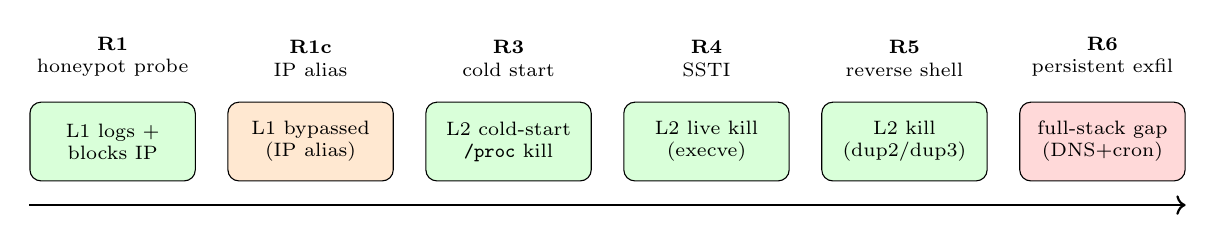
\begin{tikzpicture}[font=\footnotesize,
  oc/.style={draw, rounded corners, minimum width=2.1cm, minimum height=1.0cm,
             align=center, font=\scriptsize},
  good/.style={oc, fill=green!15}, warn/.style={oc, fill=orange!18},
  gap/.style={oc, fill=red!15}]
  \node[good] (o1) {L1 logs +\\ blocks IP};
  \node[warn, right=4mm of o1] (o2) {L1 bypassed\\ (IP alias)};
  \node[good, right=4mm of o2] (o3) {L2 cold-start\\ \texttt{/proc} kill};
  \node[good, right=4mm of o3] (o4) {L2 live kill\\ (execve)};
  \node[good, right=4mm of o4] (o5) {L2 kill\\ (dup2/dup3)};
  \node[gap,  right=4mm of o5] (o6) {full-stack gap\\ (DNS+cron)};
  \foreach \n/\r/\a in {o1/R1/honeypot probe, o2/R1c/IP alias,
                         o3/R3/cold start, o4/R4/SSTI,
                         o5/R5/reverse shell, o6/R6/persistent exfil}
     \node[above=2mm of \n, align=center, font=\scriptsize] {\textbf{\r}\\ \a};
  \draw[->,thick] ([yshift=-3mm]o1.south west) -- ([yshift=-3mm]o6.south east);
\end{tikzpicture}}
\caption{Attack--defense rounds from the defender's side. Green = attack
stopped; amber = a layer is bypassed (hand-off to the next layer); red = a gap
nothing in the stack closes. Time flows left to right.}
\label{fig:rounds}
\end{figure}

\begin{enumerate}[leftmargin=1.4em]
  \item \textbf{Recon / honeypot trap (R1--1b).} Attacker hits :2222.
        Honeypot logs the IP; network MDR inserts an \co{iptables} DROP in
        $<$1\,s; attacker's original IP loses all access. \emph{Layer 1 works.}
  \item \textbf{IP-alias bypass (R1c).} Attacker adds an alias IP and reaches
        :9999 again. \emph{Layer 1 is bypassed -- exactly as expected; hand
        off to Layer 2.}
  \item \textbf{Cold-start cleanup (R3).} Blue Team starts the eBPF MDR
        \emph{after} the agent is already running. The \co{/proc} scanner
        finds the in-memory \co{python3 /proc/<pid>/fd/<N>} agent and kills
        it; the attacker's C2 goes silent. \emph{Compensating control works.}
  \item \textbf{Real-time interception (R4).} Attacker re-runs the SSTI. The
        chain is now killed live at the \co{execve(argv)} hook (memfd is
        tainted/alerted first), so no agent ever beacons. \emph{Layer 2 hot
        path works.}
  \item \textbf{Reverse shell (R5).} Attacker switches to a TCP reverse
        shell (no memfd, no raw ICMP), so the four staging hooks stay silent
        by design. The same tool still catches it: \co{connect} raises an
        alert, and the process is killed the moment \co{dup2/dup3} redirects
        all three standard fds to the socket (\co{0x07}). \emph{Caught on the
        highest-confidence signal, no version change required.}
  \item \textbf{Persistent DNS exfiltration (R6).} A \co{crontab} planted
        earlier re-downloads an exfil agent that ships data over DNS. It uses
        only \co{socket(SOCK\_DGRAM)} + \co{sendto} -- all legitimate
        syscalls -- so the eBPF MDR raises \emph{no alert}, and the persistence
        survived every kill. \emph{Full-stack gap (\S\ref{sec:limits}).}
\end{enumerate}

\subsection{Reset between runs}
\co{cleanup.sh} returns the lab to a known-good state: it kills leftover
processes, flushes the \co{iptables} rules the MDR added, removes IP
aliases, truncates \co{trap.log}/\co{soc\_events.jsonl}, clears \co{loot/},
and removes the persistence \co{crontab}. \co{--dry} previews without acting.
Operationally this matters: a stale \co{trap.log} would make the MDR appear
unresponsive, and a surviving crontab would re-infect the next run.

% =====================================================================
\section{Evaluation and Results}
% =====================================================================

\subsection{What the defense demonstrably stops}
\begin{itemize}[leftmargin=1.4em]
  \item \textbf{Known-IP reconnaissance/return} -- blocked at Layer~1
        (sub-second), with the explicit caveat that it is bypassable.
  \item \textbf{Fileless ICMP C2} -- stopped at Layer~2 both \emph{cold}
        (\co{/proc} scan kills an already-running agent) and \emph{hot}
        (\co{execve(argv)} kill, ICMP-correlation backstop) so no beacon is
        established.
  \item \textbf{TCP reverse shell} -- stopped at the \co{dup2/dup3}
        fd-hijack, independent of the C2 port.
\end{itemize}

\subsection{Response characteristics}
The kernel kill is \emph{pre-completion}: the SIGKILL is issued inside the
\co{sys\_enter} hook, so there is no userspace polling race for the
\emph{enforcing} path. (The \emph{alerting} path -- console line and JSONL
write -- does run in userspace after the perf-buffer read, and can lag or
drop under load; see \S\ref{sec:misc-limits}.) The network block is bounded
by the MDR poll interval (default 1\,s).

\subsection{What it does \emph{not} stop}
Three techniques traverse the entire stack untouched: SSTI itself (the root
cause), DNS/ICMP exfiltration (legitimate syscalls), and \co{crontab}
persistence. These define the next section.

% =====================================================================
\section{Limitations and Open Problems}
\label{sec:limits}
% =====================================================================
This is the core of the defensive analysis: a control you cannot describe
the failure modes of is a control you do not understand.

\subsection{Network layer: IP blocking is reactive and bypassable}
\label{sec:l1-limits-detail}
Already shown in \S\ref{sec:net-limits}: the block is keyed on a value the
attacker controls. IP aliasing defeated it in seconds; NAT, proxy chains,
cloud egress, and shared-IP environments make it worse (a block can even
harm innocent co-tenants). It is signal and friction, not prevention.

\subsection{Kernel layer: legitimate-syscall covert channels are invisible}
\label{sec:exfil-limits}
The eBPF layer matches \emph{specific dangerous syscalls and arguments}. The
DNS exfiltration agent uses \co{socket(AF\_INET, SOCK\_DGRAM)} and
\co{sendto} to port~53 -- ordinary, ubiquitous syscalls with no
distinguishing argument the current hooks inspect. There is:
\begin{itemize}[leftmargin=1.4em]
  \item no \co{memfd\_create}, so no taint;
  \item no \co{SOCK\_RAW}, so the socket hook's filter
        (\co{type==SOCK\_RAW}) never matches;
  \item no \co{dup2/dup3} fd-hijack;
  \item no \co{connect} to a suspect port (DNS uses 53, and uses
        \co{sendto}, not \co{connect}).
\end{itemize}
The data is also Base32/Base64-encoded inside DNS subdomains, so even content
inspection would need DNS-aware parsing. \textbf{This is the most important
gap}: behavior-based detection that enumerates ``bad'' syscalls is blind to
malice expressed entirely through ``good'' ones. Catching it needs a
different sensor -- egress/DNS analytics, not syscall hooks.

\subsection{Temporal gap: hooks only see new syscalls}
\label{sec:gap-limits}
Tracepoints fire going forward. Anything that happened before the MDR
started is invisible to the hot path. The \co{/proc} cold-start scan
(\S\ref{sec:coldstart}) narrows this, but it is a single snapshot, it only
recognizes the two specific memfd patterns it is coded for, and a process
that has already finished its sensitive syscalls (e.g.\ already exfiltrated)
cannot be ``un-run.'' Continuous re-scanning and earlier deployment are
partial answers; the gap cannot be fully closed by a forward-looking sensor.

\subsection{False positives and whitelist tuning}
\label{sec:fp-limits}
Every enforcing hook has a benign analogue:
\begin{itemize}[leftmargin=1.4em]
  \item \co{memfd\_create} is used by Chrome, systemd, and others -- which is
        exactly why it is alert-only here, but it still adds noise.
  \item \co{execve} from \co{/proc/fd} is used by systemd \co{sd-executor};
        the tool only avoids killing it because of the filename-vs-argv
        split, a heuristic, not a guarantee.
  \item \co{dup2(fd,0/1/2)} is normal for any shell or daemon doing I/O
        redirection. The \co{0x07}-all-three requirement reduces this, but a
        legitimate program that redirects all three standard fds to one
        descriptor would be killed.
  \item the \co{suspect\_ports} list is \emph{static}; it both misses C2 on
        unlisted ports and would false-positive on a legitimate service that
        happens to use one (a reason the connect hook is alert-only).
\end{itemize}
The whitelist is per-PID and manual, which does not scale: PIDs are
recycled, and you cannot whitelist a process that does not exist yet.

\subsection{Active-response risk}
\label{sec:ar-limits}
\co{bpf\_send\_signal(SIGKILL)} on a misclassified process is itself a
denial of service -- the detector becomes the outage. There is no
quarantine, throttle, or ``confirm'' step: a single false positive on a
critical daemon is fatal to it. This is why monitor-only is the default and
why the enforcing hooks are restricted to the highest-confidence signals;
but the residual risk is real and grows with the breadth of hooks.

\subsection{Brittleness of argument matching}
\label{sec:brittle-limits}
The detections are precise, which makes them evadable:
\begin{itemize}[leftmargin=1.4em]
  \item The \co{execve} check matches the literal prefix \co{/proc/} and
        scans bytes 6--19 for \co{/fd/}. Symlinks, bind mounts, a longer PID
        pushing \co{/fd/} past byte~19, or invoking the interpreter
        differently can dodge the pattern.
  \item The \co{argv[1]} read uses a fixed pointer offset
        (\co{argv + 8}); it inspects only the second argument.
  \item The reverse-shell signal requires \emph{exactly} fd 0,1,2. An
        attacker who multiplexes I/O differently, or redirects only one fd
        and uses the socket directly, never reaches \co{0x07}.
\end{itemize}
Bounded-loop and fixed-offset parsing are forced by the verifier, but they
make the matcher a fixed target an adversary can study and step around.

\subsection{Persistence is not addressed}
\label{sec:persist-limits}
The planted \co{crontab} re-downloads and re-runs the agent on a timer and
survived every kill in the exercise, because killing a process does not
remove the mechanism that launches it. No control here watches \co{cron},
\co{systemd} units, \co{.bashrc}, or other autostart surfaces. Eradication,
not just termination, is missing.

\subsection{Monitoring-plane and operational limits}
\label{sec:misc-limits}
\begin{itemize}[leftmargin=1.4em]
  \item \textbf{Userspace alert path can drop.} The perf buffer is 256\,KB;
        under a burst, events can be lost before Python reads them. The
        enforcing kill is unaffected (it is in-kernel), but the
        \emph{record} of it may not reach the SOC.
  \item \textbf{No durable SIEM.} \co{soc\_events.jsonl} and the SSE timeline
        are flat files and an in-memory list (capped at 1000); there is no
        retention, search, alerting, or cross-host correlation.
  \item \textbf{Per-host, root, BCC-dependent.} eBPF needs root, kernel
        headers, and a runtime Clang/LLVM compile (BCC). This is heavy to
        deploy at scale and fragile across kernel versions; a CO-RE/libbpf
        build would be far more portable.
  \item \textbf{Alert fatigue.} Alert-only hooks (memfd, standalone ICMP,
        suspect connect, systemd-pattern execve) generate volume that an
        operator must triage; without scoring this erodes attention.
  \item \textbf{Encrypted payloads.} C2 content is AES-encrypted, so the
        defense can only reason about \emph{behavior}, never content --
        reinforcing that signature/content inspection is not an option here.
\end{itemize}

\subsection{Root cause is untouched}
\label{sec:rootcause}
The SSTI vulnerability (T1190) and the fact that the target runs as root are
never fixed by any of these controls -- they detect/limit \emph{consequences},
not the entry point or the blast radius. A defense that stops the agent but
leaves the injectable endpoint and root execution in place is winning rounds,
not the game.

% =====================================================================
\section{Hardening Recommendations and Future Work}
% =====================================================================
Mapped to the gaps above:
\begin{enumerate}[leftmargin=1.4em]
  \item \textbf{Close the exfiltration gap (\S\ref{sec:exfil-limits}).}
        Add an egress sensor: DNS query-rate and subdomain-entropy/length
        analytics, allow-listed resolvers, and monitoring of DNS-over-HTTPS.
        Detect ICMP payload volume/entropy anomalies. This is a different
        sensor class than syscall hooks and is the highest-value addition.
  \item \textbf{Add eradication for persistence (\S\ref{sec:persist-limits}).}
        Monitor \co{cron}, \co{systemd} units, and shell rc files; on a
        confirmed compromise, remove the launcher, not just the process.
  \item \textbf{Move from single-signal kills to scoring
        (\S\ref{sec:fp-limits}, \S\ref{sec:ar-limits}).} Correlate
        \co{connect}+\co{dup2}+new-socket-fd into a confidence score; reserve
        auto-kill for high scores and quarantine/alert otherwise. Make the
        suspect-port list dynamic.
  \item \textbf{Harden the sensor (\S\ref{sec:brittle-limits},
        \S\ref{sec:misc-limits}).} Normalize paths before matching; widen the
        argv scan; switch perf to the BPF ring buffer; rebuild on
        CO-RE/libbpf for portability and lower deploy cost.
  \item \textbf{Build a real monitoring plane.} Ship events to a durable
        SIEM with retention, search, alerting, and multi-host correlation;
        attach response playbooks to alert classes.
  \item \textbf{Fix the root cause (\S\ref{sec:rootcause}).} Patch the SSTI
        (no \co{render\_template\_string} on user input), drop the target's
        privileges from root, and add a WAF/input-validation layer so Layer~2
        is a backstop, not the only thing standing between a web request and
        kernel-level code execution.
\end{enumerate}

% =====================================================================
\section{Conclusion}
% =====================================================================
The Blue Team stack shows what layered, behavior-based defense buys you and
where it stops. Layer~1 (honeypot + \co{iptables}) produces clean, early
signal and sub-second blocking, but is reactive and trivially bypassed by an
IP change. Layer~2 (eBPF) is the real enforcement: source-IP-agnostic,
fileless-visible, and able to kill a process in kernel space before a
dangerous syscall completes -- it stopped both the fileless ICMP C2 (cold and
hot) and the TCP reverse shell at the \co{dup2/dup3} fd-hijack. Yet the same design
that makes it strong -- enumerating specific dangerous syscalls -- makes it
blind to malice built from legitimate syscalls: DNS/ICMP exfiltration and a
\co{crontab} persistence mechanism survived the entire stack. The honest
takeaway is the project's thesis stated from the defender's side:
defense-in-depth is a continuous process. Each layer is expected to fail
against some class of attack; security comes from making sure the next layer,
and the next sensor, is already watching the gap.

% =====================================================================
\appendix
\section{Blue Team Commands}
% =====================================================================
\begin{lstlisting}
# --- environment (once) ---
bash setup_env.sh
source .venv/bin/activate

# --- Layer 1: deception + network MDR ---
sudo .venv/bin/python3 target/honeypot.py
sudo .venv/bin/python3 blue_team/blue_mdr_network.py --cleanup

# --- Layer 2: kernel MDR ---
sudo .venv/bin/python3 blue_team/blue_ebpf_mdr_v2.py --kill \
     --suspect-ports 4444,4445,5555,1234,1337 \
     --whitelist <pid1>,<pid2>

# --- monitoring plane ---
python3 blue_team/soc_dashboard.py --port 8080

# --- reset between runs ---
sudo bash cleanup.sh          # add --dry to preview
\end{lstlisting}

\section{eBPF hook reference}
\begin{center}
\small
\begin{tabularx}{\linewidth}{@{}l Y@{}}
\toprule
\textbf{Tracepoint} & \textbf{Purpose}\\
\midrule
\co{sched/sched\_process\_fork} & propagate memfd taint to children\\
\co{syscalls/sys\_enter\_memfd\_create} & fileless staging (alert + taint)\\
\co{syscalls/sys\_enter\_execve} & exec from \co{/proc/fd} (kill on argv)\\
\co{syscalls/sys\_enter\_socket} & raw ICMP socket (kill if correlated)\\
\co{syscalls/sys\_enter\_connect} & connect to suspect port (alert)\\
\co{syscalls/sys\_enter\_dup2} & reverse-shell fd hijack (kill at 0x07)\\
\co{syscalls/sys\_enter\_dup3} & dup3 variant of the above (kill at 0x07)\\
\bottomrule
\end{tabularx}
\end{center}

\section{SOC event schema (\texttt{soc\_events.jsonl})}
\begin{lstlisting}
{
  "ts":       "2026-06-05 14:30:01",   // event time
  "source":   "EBPF_v2",                // EBPF_v2 | NETWORK_MDR | HONEYPOT
  "event":    "REVERSE_SHELL",          // event label
  "severity": "CRITICAL",               // CRITICAL | HIGH | MEDIUM | INFO
  "ip":       "",                        // source/target IP if applicable
  "comm":     "python3",                // process name
  "action":   "KILLED",                 // KILLED | BLOCKED | ALERT | LOGGED
  "detail":   "PID:34567 PPID:34500 ..."// free-form context
}
\end{lstlisting}

\end{document}
